\documentclass[12pt,a4paper,titlepage]{scrreprt}

% Language is defined in package module

\usepackage {fontspec}
\usepackage[hidelinks]{hyperref}
\usepackage{pdfpages} % For inclusion of PDFs

\usepackage{tabulary}
\usepackage{emoji}

%pro formátování čísel
\usepackage{numprint}
\npthousandsep{\,}\npthousandthpartsep{}\npdecimalsign{.}

%Uprava (odstraneni modifikaci generovaneneho texttu tridou scratcl)
\setkomafont{disposition}{\mdseries\rmfamily}

%\title{\vspace{6cm}Návrh zařízení pro testování nabíjecích kabelů}
%\subtitle{Bakalářská práce}
%\author{Filip Šimek}
%\date{\today}

%font
%\setmainfont{DejaVu Serif}
\setmainfont{Times_New_Roman}

%Rozestup řádku (1.5)
\linespread{1.35}

%Nastaveni okraje (normostrana)
%\usepackage[left=3.00cm, right=3.00cm, top=2.0cm, bottom=2.50cm]{geometry}
\usepackage[a4paper, left=3.50cm, right=1.50cm, top=2.50cm, bottom=2.50cm]{geometry}

%\usepackage[left=2.25cm, right=2.25cm, top=1.75cm, bottom=1.75cm, includeheadfoot]{geometry}
%\setlength{\parindent}{0pt} % Odstraní odsazení prvního odstavce každé sekce

\RedeclareSectionCommand[
  beforeskip=.1cm,
  afterskip= .1cm %1.0ex plus .2ex
]{chapter}

%Justify text mode
\tolerance=1
\emergencystretch=\maxdimen
\hyphenpenalty=10000
\hbadness=10000

% WIP modules
\usepackage{glossaries}


% My modules
% Přidá automatické zalomení spojek

%\usepackage[czech]{babel}
\usepackage{polyglossia}
\setdefaultlanguage{czech}

% Define custom hyphenation rules
%\babelhyphenation[czech]{a}
%\babelhyphenation[czech]{u}
%\babelhyphenation[czech]{i}
%\babelhyphenation[czech]{v}
%\babelhyphenation[czech]{s}
%\babelhyphenation[czech]{o}
%\babelhyphenation[czech]{proto}
%\babelhyphenation[czech]{protože}
%\babelhyphenation[czech]{je}
% Přidá article příkaz pro drobnější dělení

\makeatletter
\renewcommand\paragraph{\@startsection{paragraph}{4}{\z@}%
            {-2.5ex\@plus -1ex \@minus -.25ex}%
            {1.25ex \@plus .25ex}%
            {\normalfont\normalsize}}
\makeatother
\setcounter{secnumdepth}{4} % how many sectioning levels to assign numbers to
\setcounter{tocdepth}{4}    % how many sectioning levels to show in ToC
% Přidá custom zvýraznění v listings

\usepackage{listings}
\usepackage{xcolor}

\definecolor{codegreen}{rgb}{0,0.6,0}
\definecolor{codegray}{rgb}{0.5,0.5,0.5}
\definecolor{codepurple}{rgb}{0.58,0,0.82}
\definecolor{backcolour}{rgb}{0.95,0.95,0.92}

\lstdefinestyle{mystyle}
{
morekeywords={override}, % Add 'override' as a keyword
backgroundcolor=\color{backcolour},   
commentstyle=\color{codegreen},
keywordstyle=\color{magenta},
numberstyle=\tiny\color{codegray},
stringstyle=\color{codepurple},
basicstyle=\footnotesize,
breakatwhitespace=false,         
breaklines=true,                 
captionpos=b,                    
keepspaces=true,                 
numbers=left,                    
numbersep=5pt,                  
showspaces=false,                
showstringspaces=false,
showtabs=false,                  
tabsize=2,
escapeinside=``
}

\lstset
{
morekeywords={override}, % Add 'override' as a keyword
style=mystyle
}
% Přidá tabulky++

\usepackage{multirow}
\usepackage{makecell}
\usepackage{array}

% My commands
\newcommand{\ardMeg}{Arduino Mega 2560}
%!TeX root =  ../thesis.tex

\makeglossaries

\newglossaryentry{keyword1}{
    name={Keyword 1},
    description={Description of Keyword 1}
}

\newglossaryentry{keyword2}{
    name={Keyword 2},
    description={Description of Keyword 2}
}

\newglossaryentry{ard}{
    name={Arduino},
    description={IoT device}
}

\newglossaryentry{ard2}{
    name={Arduino2},
    description={IoT device2}
}

\makeglossaries

\begin{document}

	%\includepdf{specialPages/frontPage/frontPage.pdf} %Desky
	\includepdf{specialPages/titlePage/titlePage.pdf} %\maketitle 
	\includepdf[pages={1-2}]{specialPages/zadaniBP.pdf}
	
	%!TeX root =  ../thesis.tex

Prohlašuji: \\
Práci s názvem “Návrh zařízení pro testování nabíjecích kabelů” jsem vypracoval samostatně. Veškeré literární prameny a informace, které jsem v práci využil, jsou uvedeny v seznamu použité literatury.
Byl jsem seznámen s tím, že se na moji práci vztahují práva a povinnosti vyplývající ze zákona č. 121/2000 Sb., o právu autorském, o právech souvisejících s právem autorským a o změně některých zákonů (autorský zákon), ve znění pozdějších předpisů, zejména se skutečností, že Univerzita Pardubice má právo na uzavření licenční smlouvy o užití této práce jako školního díla podle § 60 odst. 1 autorského zákona, a s tím, že pokud dojde k užití této práce mnou nebo bude poskytnuta licence o užití jinému subjektu, je Univerzita Pardubice oprávněna ode mne požadovat přiměřený příspěvek na úhradu nákladů, které na vytvoření díla vynaložila, a to podle okolností až do jejich skutečné výše.

Beru na vědomí, že v souladu s § 47b zákona č. 111/1998 Sb., o vysokých školách a o změně a doplnění dalších zákonů (zákon o vysokých školách), ve znění pozdějších předpisů, a směrnicí Univerzity Pardubice č. 7/2019 Pravidla pro odevzdávání, zveřejňování a formální úpravu závěrečných prací, ve znění pozdějších dodatků, bude práce zveřejněna prostřednictvím Digitální knihovny Univerzity Pardubice.

V Pardubicích dne \hfill Filip Šimek v. r. 2024
	\thispagestyle{empty}
	%!TeX root =  ../thesis.tex
\clearpage
\vspace*{\fill}
\section*{Poděkování}
Mé poděkování patří vedoucímu bakalářské práce Ing. Janu Fikejzovi, Ph.D. za odborné vedení, trpělivost, ochotu a veškerý věnovaný čas, který mi v průběhu zpracování bakalářské práce věnoval. Dále bych chtěl poděkovat rodině a svým kamarádům, kteří mi byli po celou dobu studia oporou.
	\thispagestyle{empty}
	
	\setcounter{page}{5}
	\printglossary
	\thispagestyle{empty}
	
	\listoffigures
	\addcontentsline{toc}{section}{Seznam obrázků}
	\thispagestyle{empty}
	\listoftables
	\addcontentsline{toc}{section}{Seznam tabulek}
	\thispagestyle{empty}

	\addtocontents{toc}{\protect\pagestyle{empty}}
	\addtocontents{toc}{\protect\thispagestyle{empty}}
	\tableofcontents
	\thispagestyle{empty}

	
	\chapter{Úvod}
	Téma mojí bakalářské práce je “Návrh zařízení pro testování nabíjecích kabelů”. Toto zařízení bude řízeno jednodeskovým počítačem Arduino (\ardMeg) a bude se testovat a následně používat v reálném prostředí. Tudíž má má bakalářská práce i praktické využití a není jen teoretická. Ovšem součástí je teoretická část o IoT - Internet of Things neboli Internet věcí. \gls{ard}
	
	
	\chapter{IoT - Internet věcí}
	%!TeX root =  thesis.tex

\section{Úvod do IoT}

\section{Jednodeskové počítače v kontextu IoT}
% Tato sekce by měla obsahovat informace o různých typech jednodeskových počítačů (např. Raspberry Pi, Arduino) a jejich využití v IoT.

\subsection{Raspberry Pi}
% Podsekce popisující vlastnosti a možnosti Raspberry Pi v IoT.

\subsection{Arduino}
% Podsekce popisující vlastnosti a možnosti Arduino v IoT.
\subsection{Arduino vs. Raspberry Pi}

\section{Technologie v IoT}
% V této části popište různé technologie a protokoly používané v IoT, jako je MQTT, CoAP, Zigbee, BLE atd.

\subsection{MQTT}
% Podsekce popisující MQTT a jeho využití v IoT.

\subsection{CoAP}
% Podsekce popisující CoAP a jeho využití v IoT.

\subsection{Zigbee}
% Podsekce popisující Zigbee a jeho využití v IoT.

\subsection{BLE (Bluetooth Low Energy)}
% Podsekce popisující BLE a jeho využití v IoT.

\section{Výzvy v IoT}
% Zde popište výzvy spojené s implementací a provozem IoT systémů, jako je zabezpečení, škálovatelnost, interoperabilita atd.
	
	
	\chapter{Použitý HW a SW}
	%!TeX root =  ../../thesis.tex

\section{Arduino}
Základem testeru je mikrokontrolér od značky Arduino model \ardMeg. Tento model disponuje velkým počtem pinům, na které je možné připojit různá zařízení a následně je ovládat mikrokontrolérem. Mikrokontroléry Arduino se programují pomocí C/C++. Já firmware pro toto tester píši v C++.

\begin{figure}[h!]
	\centering
	
\includegraphics[width=\textwidth]{pictures/placeHolderFHD.png}
    	\caption{\ardMeg}
   	\label{fig:arduinoMega}
\end{figure}


%\subsection*{Ino file}
%\lstinputlisting[language=C++, caption={Code.ino}, label={lst:code}]{../code/Code.ino}

%\subsubsection*{Co je to Ino file?}
%Ino file je soubor skatche pro Arduino, Arduino IDE ho využívá jako hlavní soubor, jen má místo metody main() metody setup() a loop().  Metoda setup() slouží pro přípravu zařízení a je automaticky volána při spuštění zaříze,  loop() pak obsahuje kód, který je vykonáván %mikrokontrolérem, dokud není vypnut nebo se nevyskytne problém. Arduino se dá programovat i pomocí svého upraveného jazyka C++, proto koncovka .ino.




	%!TeX root =  ../thesis.tex

\section{IComponent}
\lstinputlisting[language=C++, caption={IComponent}, label={lst:cpp_icomp}]{../code/src/components/IComponent.h}

%!TeX root =  ../../thesis.tex

\section{Display}

Pro potřeby testeru byl vybrán standardní LCD displej se žlutým podsvícením o čtyřech řádcích po dvaceti znacích. Tento displej bude postačovat, jelikož je potřeba zobrazit menu, aby uživatel mohl vybrat typ kabelu dle koncových konektorů a následně výsledek testu, kterému jsou věnovány poslední dva řádky, na které se taky budou vypisovat chybová hlášení. V prvním řádku je vypsána verze programu a na poslední pozici bliká znak “\#”, který se objeví a zmizí vždy na jednu sekundu, z důvodu kontroly, že zařízení “nezamrzlo” a je možné jej bez problému použít.

\begin{figure}[H]
	\centering
	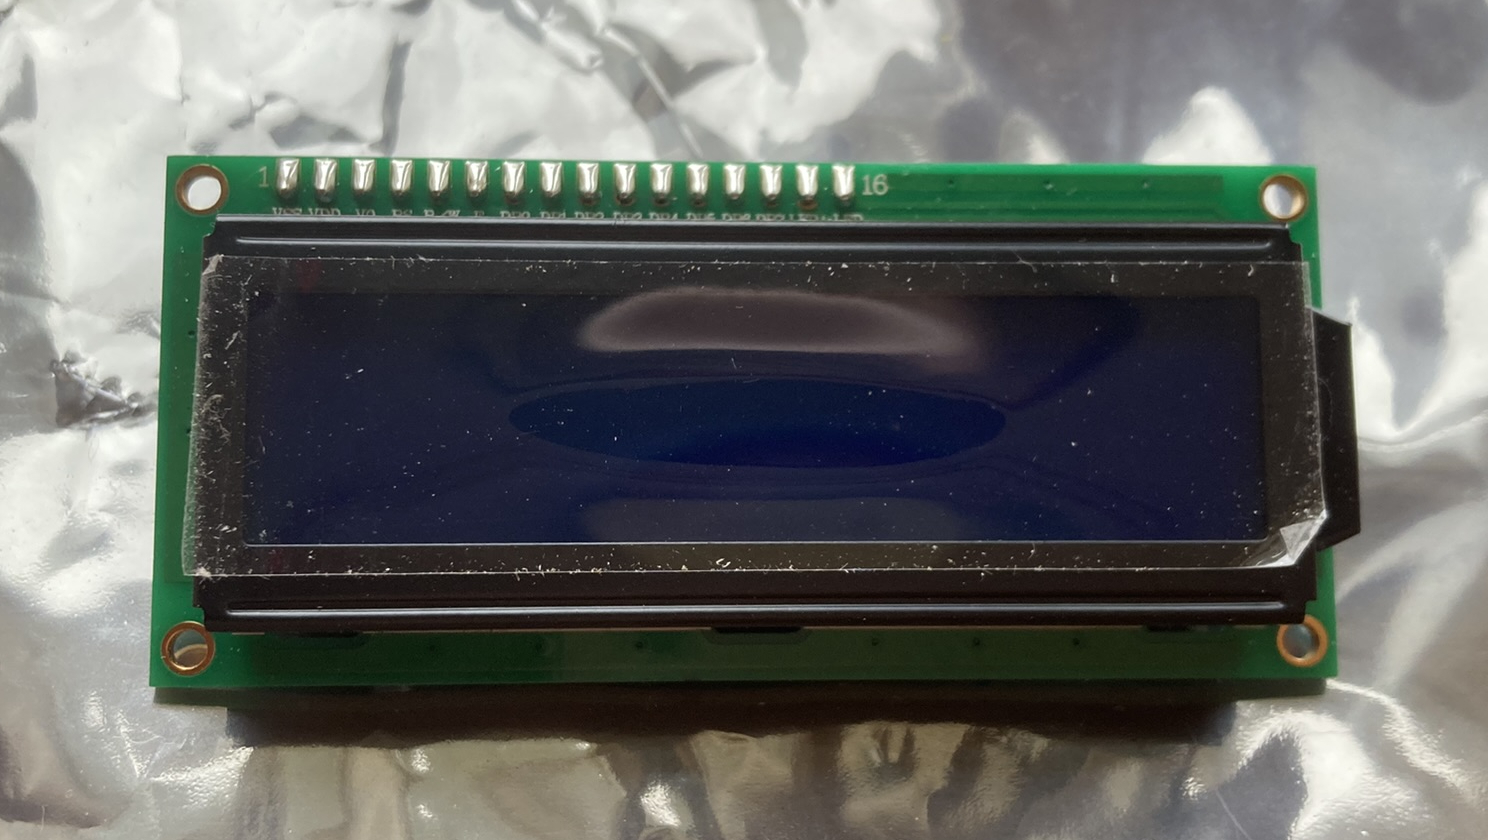
\includegraphics[width=0.9\textwidth]{pictures/display.jpeg}
    	\caption{Display}
   	\label{fig:displayHW}
\end{figure}

Na obrázku \ref{fig:displayHW} je displej, který sice není použitý pro tester, ale je to principiálně stejný displej a vlevo nahoře jsou vidět vrchní strany pinů, kterými se displej připojuje k Arduino nebo po případě k breadbordu.
%!TeX root =  ../../thesis.tex

\section{Klávesnice}
\begin{figure}[h!]
	\centering
	
\includegraphics[width=\textwidth]{pictures/placeHolderFHD.png}
    	\caption{Klávesnička}
   	\label{fig:keyborad}
\end{figure}

\subsection{Připojení k desce}
\begin{table} [h!]
	\centering
	\catcode`\-=12 % Because of czech
	\begin{tabular}[c]{|| c | c | c ||}
	\hline
		\multicolumn{3}{||c||}{Piny klávesničky} \\
	\hline
 		 \textbf{PIN} & \textbf{Tlačítko} & \textbf{Akce}\\
	\hline
		42 &  RIGHT & Posune menu doprava\\
	\hline
		46 & POWER & N/A\\
	\hline
		48 & LEFT & Posune menu doleva\\
	\hline
		50 & MENU & N/A\\
	\hline
		52 & AUTO & Začne testovat vybraný kabel\\
	\hline
	\end{tabular}
	\caption{Pinové rozložení klávesnice}
	\label{table:pinKB}
\end{table}

\newpage
\subsection{Keyboard controller}
\lstinputlisting[language=C++, caption={Display controller}, label={lst:cpp_display}]{../code/src/components/Keyboard.h}

	%!TeX root =  ../thesis.tex

\section{IO Panel}
\begin{figure}[h!]
	\centering
	
\includegraphics[width=\textwidth]{pictures/placeHolderFHD.png}
    	\caption{IO Panel}
   	\label{fig:panelIO}
\end{figure}

\newpage
\section{IConnector}
\lstinputlisting[language=C++, caption={Connector}, label={lst:cpp_Connector}, style=riyuCpp]{../code/src/deviceIO/Connector.h}
Toto je společný předek pro jednotlivé konektory, který nám usnadní manipulaci s jeho potomky, tedy již specifickými konektory.

%!TeX root =  ../../thesis.tex

\section{XLR 3}
\subsection{Pinové zapojení}
\begin{table} [h!]
	\centering
	\catcode`\-=12 % Because of czech
	\begin{tabular}[c]{|| c | c ||}
	\hline
		\multicolumn{2}{||c||}{XLR-3 In} \\
	\hline
 		 \textbf{PIN} & \textbf{Akce}\\
	\hline
		22 &  Uzemění\\
	\hline
		24 & Positive polarity terminal for balanced audio circuits \\
	\hline
		N/A & Negative polarity terminal for balanced circuits \\
	\hline
	\end{tabular}
	\caption{Pinové rozložení XLR 3 - In}
	\label{table:pinXLR-IN}
\end{table}

\begin{table} [h!]
	\centering
	\catcode`\-=12
	\begin{tabular}[c]{|| c | c ||}
	\hline
		\multicolumn{2}{||c||}{XLR-3 Out} \\
	\hline
 		 \textbf{PIN} & \textbf{Akce}\\
	\hline
		26 &  Uzemění\\
	\hline
		28 & Positive polarity terminal for balanced audio circuits \\
	\hline
		N/A & Negative polarity terminal for balanced circuits \\
	\hline
	\end{tabular}
	\caption{Pinové rozložení XLR 3 - Out}
	\label{table:pinXLR-OUT}
\end{table}
%!TeX root =  ../../thesis.tex

\section{Jack 2.1}

\subsection{Pinové zapojení}
\begin{table} [h!]
	\centering
	\catcode`\-=12
	\begin{tabular}[c]{|| c | c ||}
	\hline
		\multicolumn{2}{||c||}{Jack 2.1} \\
	\hline
 		 \textbf{PIN} & \textbf{Akce}\\
	\hline
		30 &  ?\\
	\hline
		31 & ? \\
	\hline
	\end{tabular}
	\caption{Pinové rozložení Jack 2.1}
	\label{table:pinJack21}
\end{table}
%!TeX root =  ../../thesis.tex

\section{Jack 2.5}
\subsection{Pinové zapojení}
\begin{table} [h!]
	\centering
	\catcode`\-=12
	\begin{tabular}[c]{|| c | c ||}
	\hline
		\multicolumn{2}{||c||}{Jack 2.5} \\
	\hline
 		 \textbf{PIN} & \textbf{Akce}\\
	\hline
		32 &  ?\\
	\hline
		33 & ? \\
	\hline
	\end{tabular}
	\caption{Pinové rozložení Jack 2.5}
	\label{table:pinJack25}
\end{table}

%!TeX root =  ../../thesis.tex

\section{RCA}
\subsection{Pinové zapojení}
\begin{table} [h!]
	\centering
	\catcode`\-=12
	\begin{tabular}[c]{|| c | c ||}
	\hline
		\multicolumn{2}{||c||}{RCA} \\
	\hline
 		 \textbf{PIN} & \textbf{Akce}\\
	\hline
		34 &  ?\\
	\hline
		35 & ? \\
	\hline
	\end{tabular}
	\caption{Pinové rozložení RCA}
	\label{table:pinRCA}
\end{table}

%\include{chapters/connectors/bosh.tex}
%\include{chapters/connectors/shimano.tex}

	
	\chapter{Návrh testeru kabelů – Hardwarová část}
	%!TeX root =  ../../thesis.tex

\section{Tester}
Tester je umístěn v plastovém boxu na vrchní části je umístěn displej a klávesnice na ovládání a na přední části jsou konektory pro testovaní kabelů.\\

Na obrázku \ref{fig:tester}  je pohled na výsledné testovací zařízení z vrchu, kdy je vidět celé ovládací rozhraní.
\\
Obrázek \ref{fig:testerIO} ukazuje konektory, kdy první tři zleva jsou výstupní a zbylé jsou vstupní, neboli ty testované.

\begin{figure}[H]
	\centering
	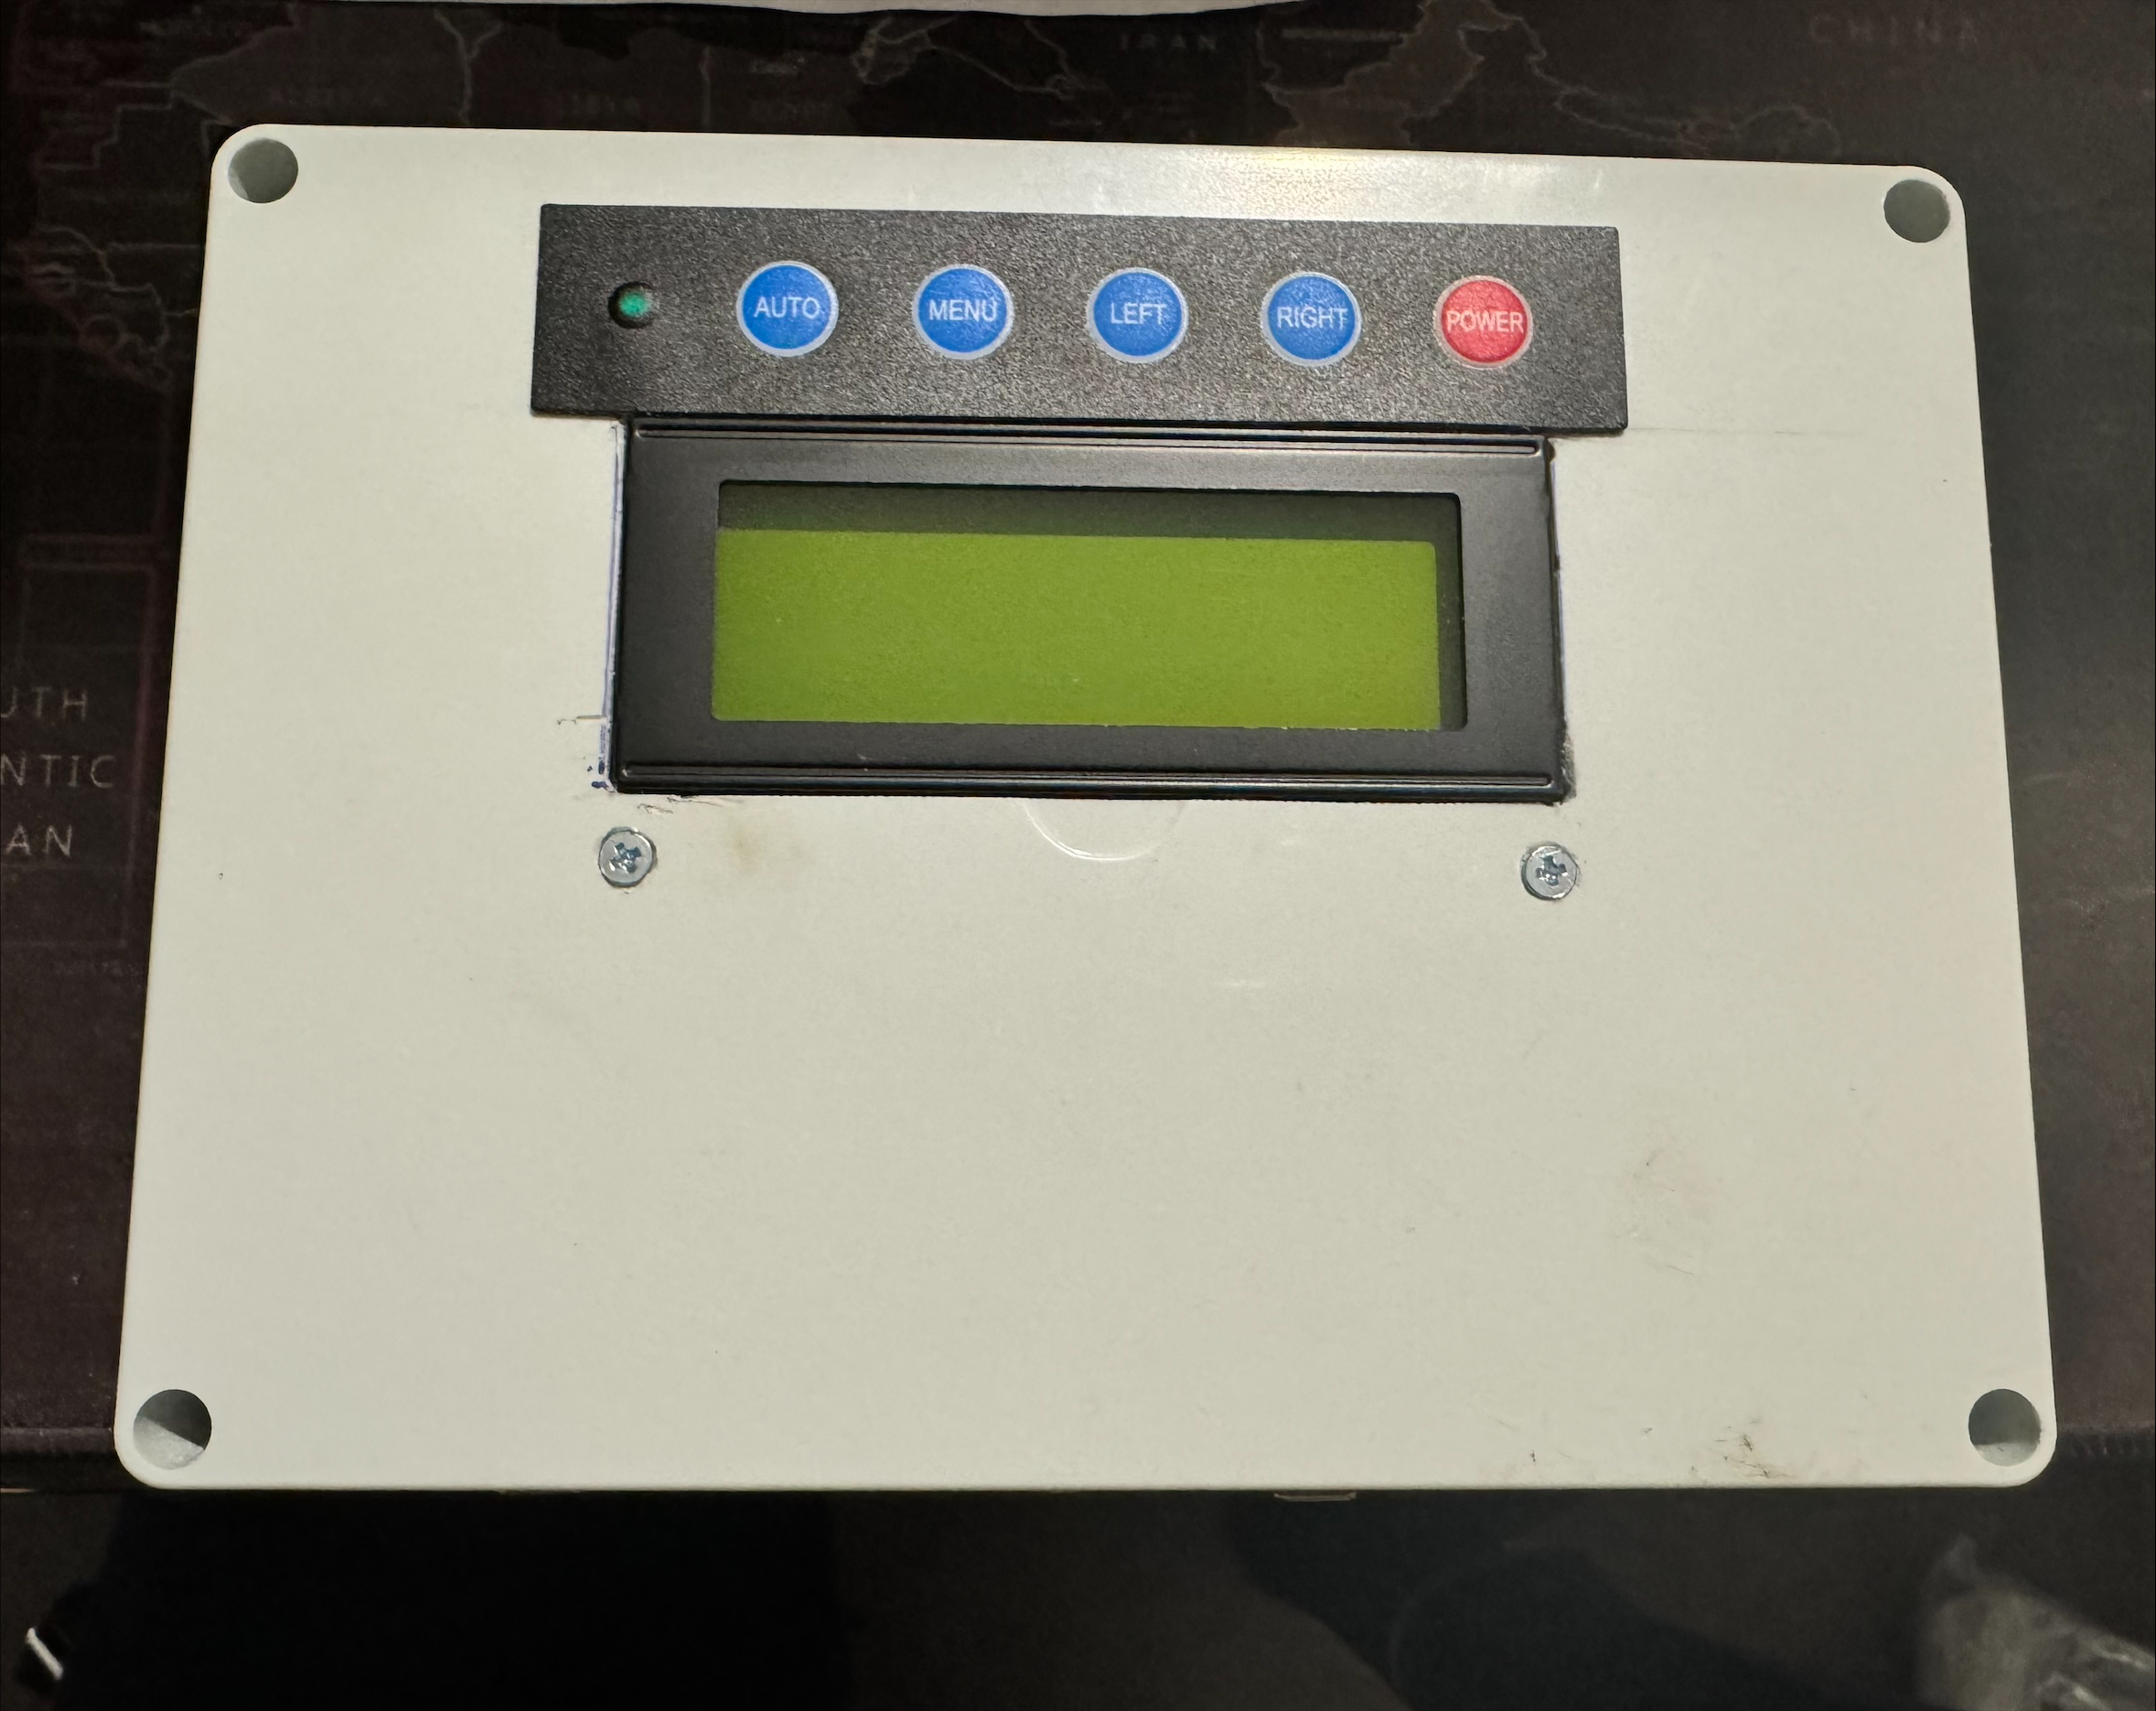
\includegraphics[width=0.9\textwidth]{pictures/tester-top.jpeg}
    	\caption{Výsledný tester na kabely}
   	\label{fig:tester}
\end{figure}

\begin{figure}[H]
	\centering
	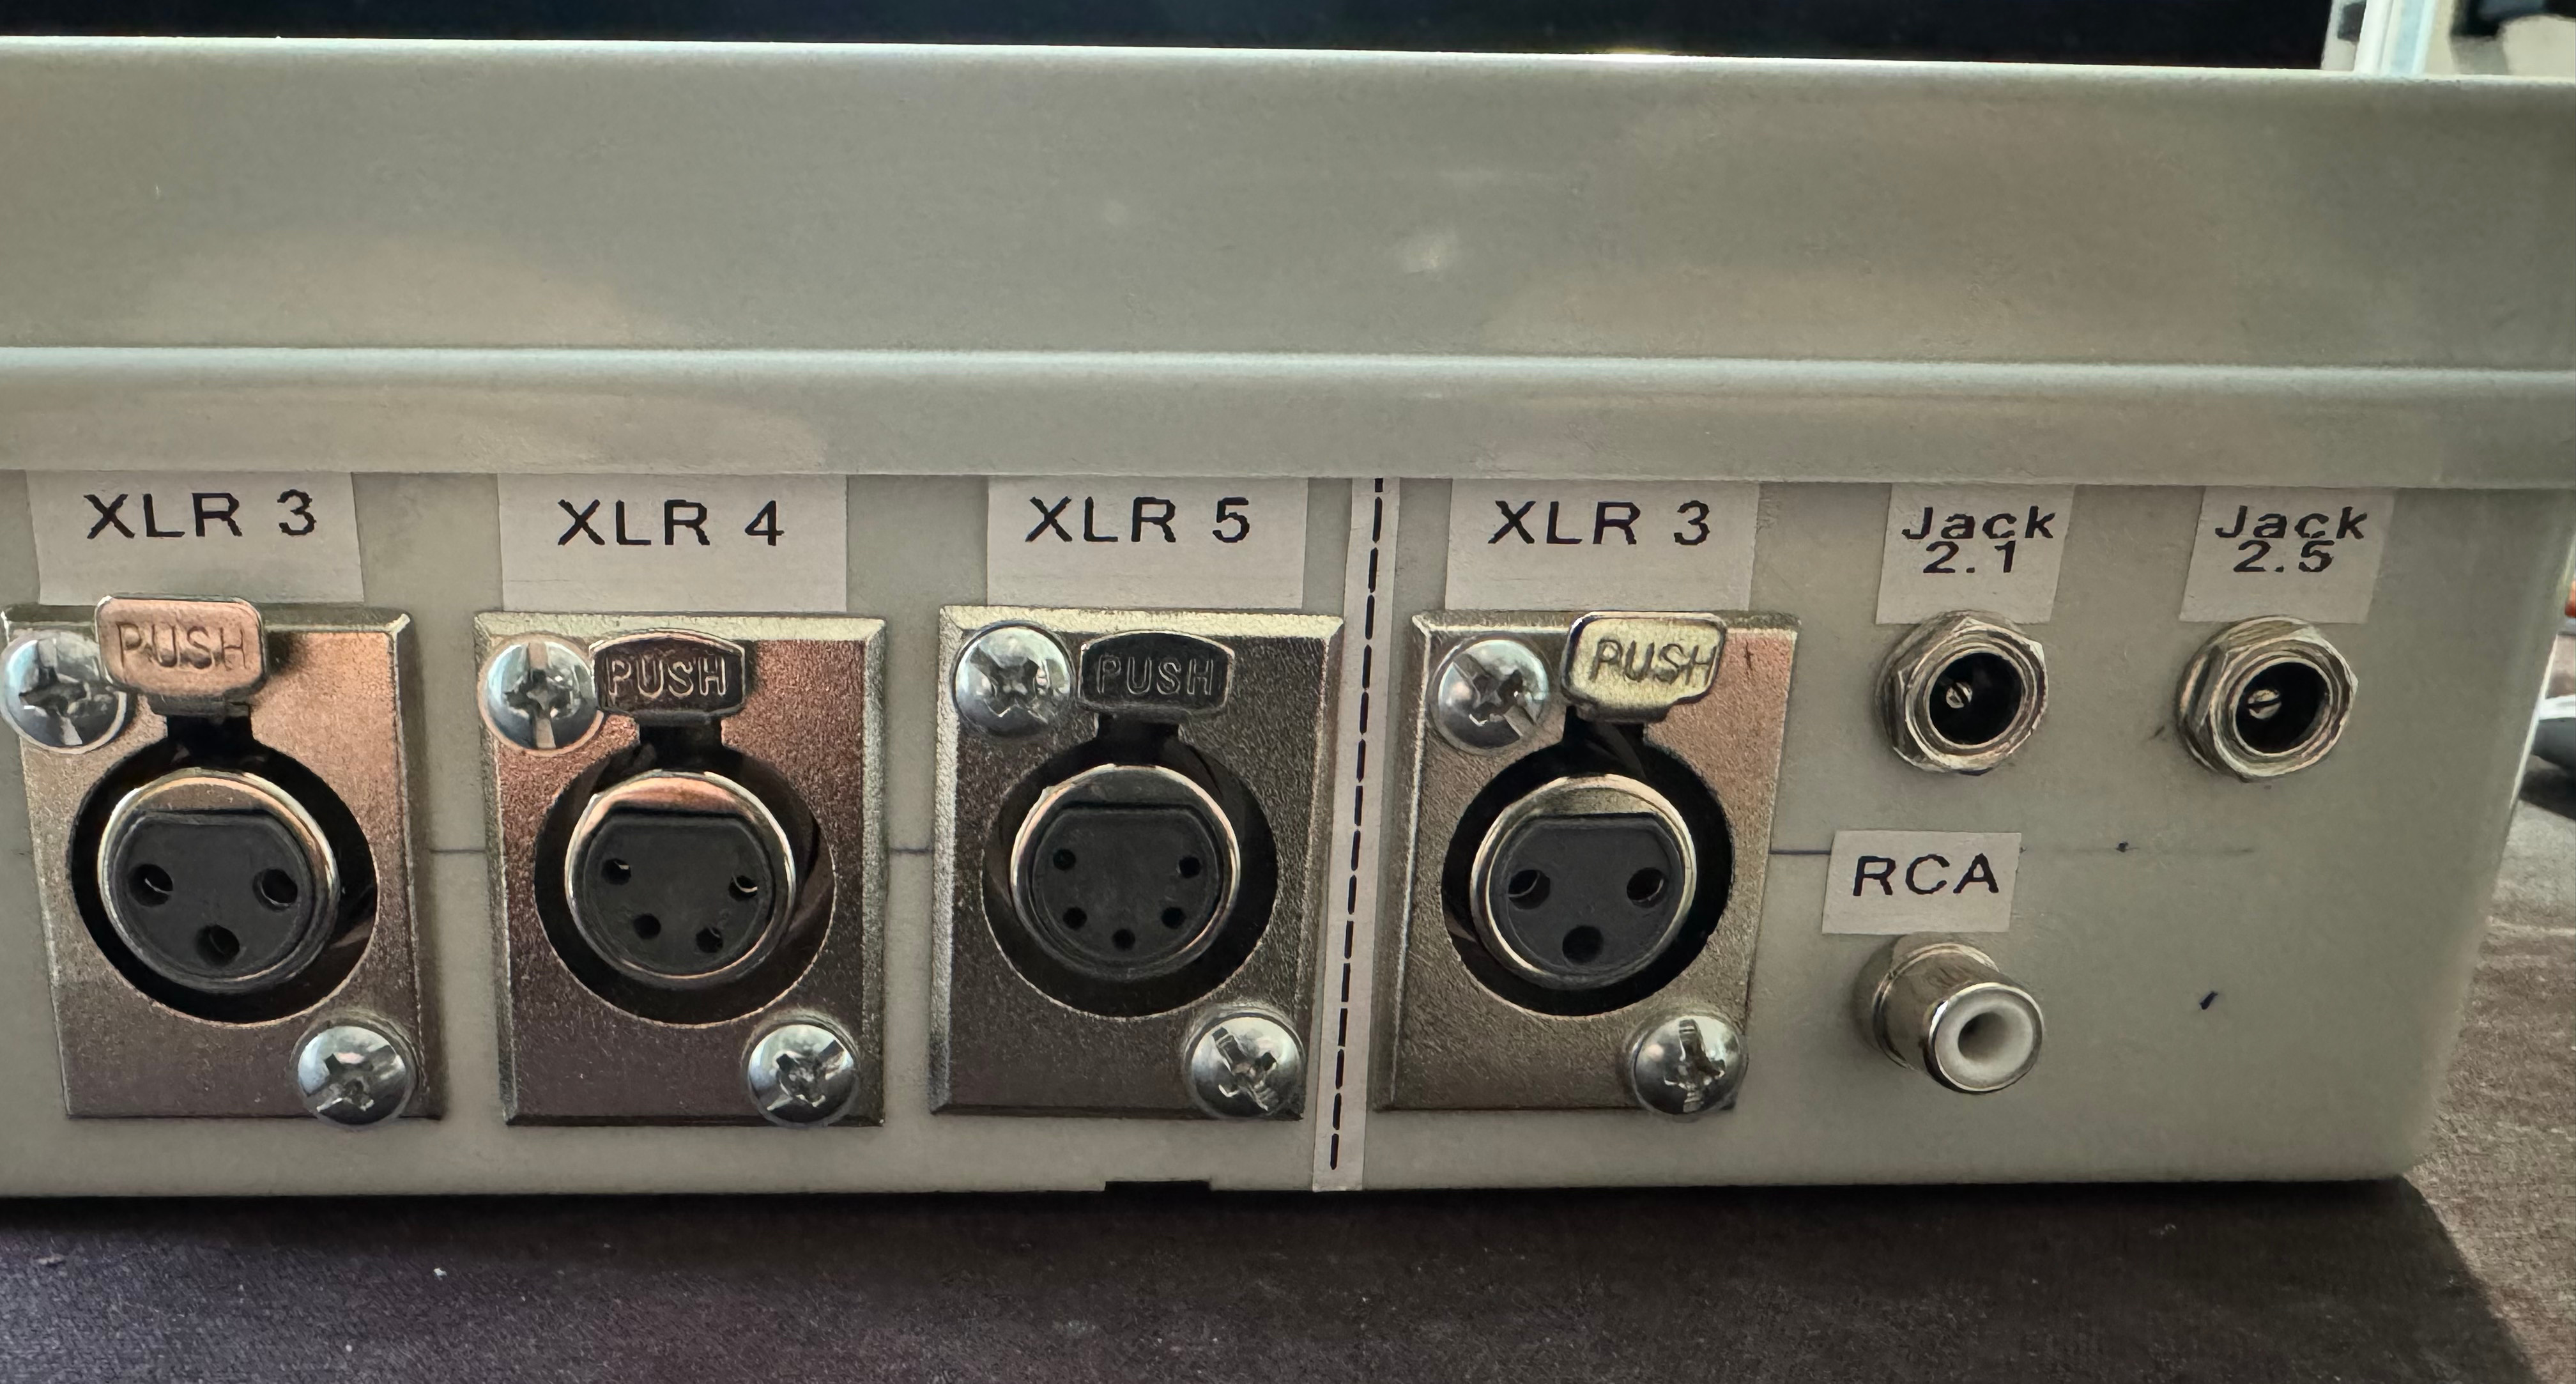
\includegraphics[width=0.9\textwidth]{pictures/tester-io.jpeg}
    	\caption{Výsledný tester na kabely}
   	\label{fig:testerIO}
\end{figure}


	
	\chapter{Návrh testeru kabelů – Softwarová část}
	%!TeX root =  ../../thesis.tex

\section{UML}

\section{Klíčové třídy}
\subsection{Controller}
Controller je hlavní třída, ačkoliv je hlavní část je v code.ino \ref{lst:code}, třída Controller zpřehlední kód, jelikož se do ní nic nedoplňuje při kompilaci, jako do hlavního ino souboru.

\subsection{Connector}
Společný předek pro konkrétní konektory.

\subsection{IComponent}
Společný předek pro komponenty zařízení, jako jsou například: displej, klávesnice nebo bzučák.

	
	
	\chapter{Testování}
	
	
	\chapter{Závěr}
	Závěrem je že C++ > C\#.

	\newpage
	\chapter{Přílohy}
	\section*{Zdroje}
	\addcontentsline{toc}{section}{Seznam zdrojů}
	%\lstlistoflistings
	%\addcontentsline{toc}{section}{Seznam zdrojových kódů} % Add the list of listings to the TOC as a section

\end{document}